\documentclass[11pt, a4paper]{article}\usepackage[]{graphicx}\usepackage[]{xcolor}
% maxwidth is the original width if it is less than linewidth
% otherwise use linewidth (to make sure the graphics do not exceed the margin)
\makeatletter
\def\maxwidth{ %
  \ifdim\Gin@nat@width>\linewidth
    \linewidth
  \else
    \Gin@nat@width
  \fi
}
\makeatother

\definecolor{fgcolor}{rgb}{0.345, 0.345, 0.345}
\newcommand{\hlnum}[1]{\textcolor[rgb]{0.686,0.059,0.569}{#1}}%
\newcommand{\hlsng}[1]{\textcolor[rgb]{0.192,0.494,0.8}{#1}}%
\newcommand{\hlcom}[1]{\textcolor[rgb]{0.678,0.584,0.686}{\textit{#1}}}%
\newcommand{\hlopt}[1]{\textcolor[rgb]{0,0,0}{#1}}%
\newcommand{\hldef}[1]{\textcolor[rgb]{0.345,0.345,0.345}{#1}}%
\newcommand{\hlkwa}[1]{\textcolor[rgb]{0.161,0.373,0.58}{\textbf{#1}}}%
\newcommand{\hlkwb}[1]{\textcolor[rgb]{0.69,0.353,0.396}{#1}}%
\newcommand{\hlkwc}[1]{\textcolor[rgb]{0.333,0.667,0.333}{#1}}%
\newcommand{\hlkwd}[1]{\textcolor[rgb]{0.737,0.353,0.396}{\textbf{#1}}}%
\let\hlipl\hlkwb

\usepackage{framed}
\makeatletter
\newenvironment{kframe}{%
 \def\at@end@of@kframe{}%
 \ifinner\ifhmode%
  \def\at@end@of@kframe{\end{minipage}}%
  \begin{minipage}{\columnwidth}%
 \fi\fi%
 \def\FrameCommand##1{\hskip\@totalleftmargin \hskip-\fboxsep
 \colorbox{shadecolor}{##1}\hskip-\fboxsep
     % There is no \\@totalrightmargin, so:
     \hskip-\linewidth \hskip-\@totalleftmargin \hskip\columnwidth}%
 \MakeFramed {\advance\hsize-\width
   \@totalleftmargin\z@ \linewidth\hsize
   \@setminipage}}%
 {\par\unskip\endMakeFramed%
 \at@end@of@kframe}
\makeatother

\definecolor{shadecolor}{rgb}{.97, .97, .97}
\definecolor{messagecolor}{rgb}{0, 0, 0}
\definecolor{warningcolor}{rgb}{1, 0, 1}
\definecolor{errorcolor}{rgb}{1, 0, 0}
\newenvironment{knitrout}{}{} % an empty environment to be redefined in TeX

\usepackage{alltt}

\usepackage[top = 0.7 in, bottom = 0.7 in, left = 1 in, right = 1 in]{geometry}

\usepackage{amsmath, amssymb, amsfonts}
\usepackage{enumerate}
\usepackage{array}
\usepackage{multirow}
\usepackage{dingbat}
\usepackage{fontawesome5}
\usepackage{tasks}
\usepackage{bbding}
\usepackage{twemojis}
% how to use bull's eye ----- \scalebox{2.0}{\twemoji{bullseye}}
\usepackage{fontspec}
\usepackage{customdice}
% how to put dice face ------ \dice{2}

\title{MSMS 206 : Practical 03}
\author{Ananda Biswas}
\date{\today}

\newfontface\myfont{Myfont1-Regular.ttf}[LetterSpace=0.05em]
% how to use ---- {\setlength{\spaceskip}{1em plus 0.5em minus 0.5em} \fontsize{17}{20}\myfont --write text here-- \par}

\newfontface\cbfont{CaveatBrush-Regular.ttf}
% how to use --- \myfont --write text here--
\IfFileExists{upquote.sty}{\usepackage{upquote}}{}
\begin{document}

\maketitle


\section*{\faArrowAltCircleRight[regular] \textcolor{blue}{Objective}}

\hspace{1cm} $X_1, X_2, \ldots , X_{n} \overset{\text{iid}}{\sim} Exp(\text{mean} = \theta).$


\begin{enumerate}[(i)]
\item Using CLT we have to show that $\bar{X}$ is a CAN estimator for $\theta$.
\item We also have to obtain a CAN estimator for $P[X > t] = e^{-t / \theta}$ and its asymptotic variance.
\end{enumerate}



\section*{\faArrowAltCircleRight[regular] \textcolor{blue}{Theory, R Program, Plot and Interpretation}}

\leftpointright \hspace{0.5cm} First we shall show that $\bar{X}$ is a consistent estimator for $\theta$ $i.e.$ $P[|\bar{X_n} - \theta| < \epsilon]$ tends to 1 as sample size $n$ increases. \\

We generate 10000 samples of size $n$ and calculate the relative frequency of $[|\bar{X_n} - \theta| < \epsilon]$, this is the probability obtained by empirical approach. As sample size $n$ increases, the empirical probability converges to 1. \\

We consider $\theta = 2$.

\begin{knitrout}
\definecolor{shadecolor}{rgb}{0.969, 0.969, 0.969}\color{fgcolor}\begin{kframe}
\begin{alltt}
\hldef{theta} \hlkwb{<-} \hlnum{2}
\end{alltt}
\end{kframe}
\end{knitrout}

\begin{knitrout}
\definecolor{shadecolor}{rgb}{0.969, 0.969, 0.969}\color{fgcolor}\begin{kframe}
\begin{alltt}
\hldef{prob} \hlkwb{<-} \hlkwa{function}\hldef{(}\hlkwc{size}\hldef{,} \hlkwc{epsilon}\hldef{)\{}

  \hldef{sample_list} \hlkwb{<-} \hlkwd{list}\hldef{()}

  \hlkwa{for}\hldef{(i} \hlkwa{in} \hlnum{1}\hlopt{:}\hlnum{10000}\hldef{)\{}
    \hldef{sample_list[[i]]} \hlkwb{<-} \hlkwd{rexp}\hldef{(size,} \hlkwc{rate} \hldef{=} \hlnum{1} \hlopt{/} \hldef{theta)}
  \hldef{\}}

  \hldef{x_bar} \hlkwb{<-} \hlkwd{sapply}\hldef{(sample_list, mean)}

  \hldef{m} \hlkwb{<-} \hlkwd{length}\hldef{(}\hlkwd{which}\hldef{(}\hlkwd{abs}\hldef{(x_bar} \hlopt{-} \hldef{theta)} \hlopt{<} \hldef{epsilon))}

  \hlkwd{return}\hldef{(m}\hlopt{/}\hlnum{10000}\hldef{)}
\hldef{\}}
\end{alltt}
\end{kframe}
\end{knitrout}

Here we take $\epsilon = 0.5$.

\begin{knitrout}
\definecolor{shadecolor}{rgb}{0.969, 0.969, 0.969}\color{fgcolor}\begin{kframe}
\begin{alltt}
\hldef{probs} \hlkwb{<-} \hlkwd{c}\hldef{()}

\hlkwa{for} \hldef{(i} \hlkwa{in} \hlkwd{seq}\hldef{(}\hlnum{10}\hldef{,} \hlnum{300}\hldef{,} \hlnum{5}\hldef{)) \{}
  \hldef{probs} \hlkwb{<-} \hlkwd{append}\hldef{(probs,} \hlkwd{prob}\hldef{(}\hlkwc{size} \hldef{= i,} \hlkwc{epsilon} \hldef{=} \hlnum{0.5}\hldef{))}
\hldef{\}}
\end{alltt}
\end{kframe}
\end{knitrout}



\begin{knitrout}
\definecolor{shadecolor}{rgb}{0.969, 0.969, 0.969}\color{fgcolor}\begin{kframe}
\begin{alltt}
\hldef{df1} \hlkwb{<-} \hlkwd{data.frame}\hldef{(}\hlkwc{sample_size} \hldef{=} \hlkwd{seq}\hldef{(}\hlnum{10}\hldef{,} \hlnum{300}\hldef{,} \hlnum{5}\hldef{),} \hlkwc{probability} \hldef{= probs)}

\hldef{df1} \hlopt
  \hlkwd{ggplot}\hldef{(}\hlkwd{aes}\hldef{(}\hlkwc{x} \hldef{= sample_size,} \hlkwc{y} \hldef{= probability))} \hlopt{+}
  \hlkwd{geom_point}\hldef{(}\hlkwc{size} \hldef{=} \hlnum{2}\hldef{,} \hlkwc{col} \hldef{=} \hlsng{"red"}\hldef{)} \hlopt{+}
  \hlkwd{labs}\hldef{(}\hlkwc{x} \hldef{=} \hlsng{"Sample Size"}\hldef{,} \hlkwc{y} \hldef{=} \hlsng{"Probability"}\hldef{,}
       \hlkwc{title} \hldef{=} \hlsng{"Convergence in Probability"}\hldef{)}
\end{alltt}
\end{kframe}
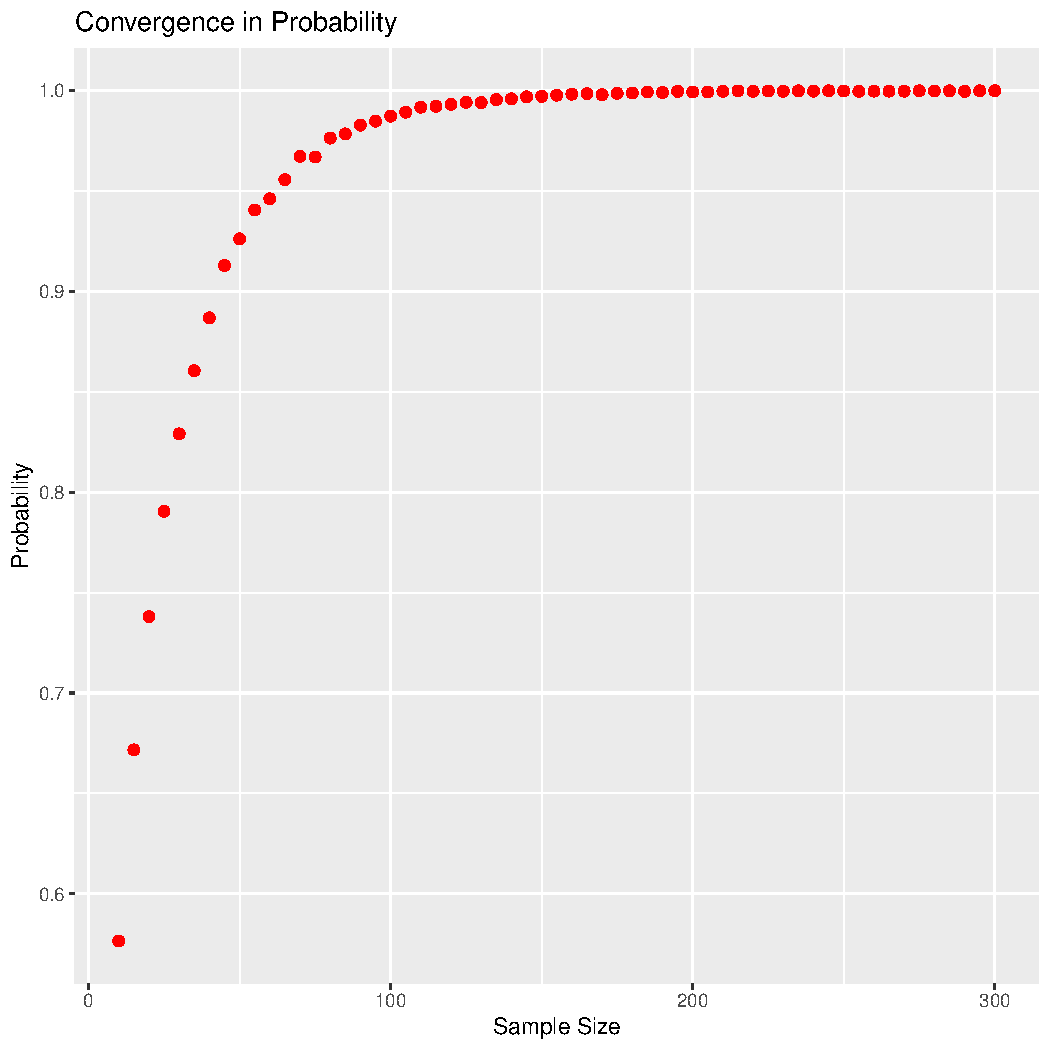
\includegraphics[width=\maxwidth]{figure/unnamed-chunk-5-1} 
\end{knitrout}

\smallpencil {\setlength{\spaceskip}{1em plus 0.5em minus 0.5em} \fontsize{17}{20}\myfont As sample size increases, the probability converges to 1. This implies that the sample mean is a consistent estimator of $\theta$. \par}


\leftpointright \hspace{0.5cm} Now we shall show that $\bar{X_n}$ has an asymptotic normal distribution. \\

We generate 10000 samples of size $n$, from there we get 10000 $\bar{X_n}$. We plot their histogram along with density curve. As sample size $n$ increases, the density curve resembles that of a normal distribution.

\newpage

First we take $n = 2$.

\begin{knitrout}
\definecolor{shadecolor}{rgb}{0.969, 0.969, 0.969}\color{fgcolor}\begin{kframe}
\begin{alltt}
\hldef{sample_list} \hlkwb{<-} \hlkwd{list}\hldef{(); size} \hlkwb{<-} \hlnum{2}

\hlkwa{for}\hldef{(i} \hlkwa{in} \hlnum{1}\hlopt{:}\hlnum{10000}\hldef{)\{}
  \hldef{sample_list[[i]]} \hlkwb{<-} \hlkwd{rexp}\hldef{(size,} \hlkwc{rate} \hldef{=} \hlnum{1} \hlopt{/} \hldef{theta)}
\hldef{\}}

\hldef{x_bar} \hlkwb{<-} \hlkwd{sapply}\hldef{(sample_list, mean)}
\end{alltt}
\end{kframe}
\end{knitrout}

\begin{knitrout}
\definecolor{shadecolor}{rgb}{0.969, 0.969, 0.969}\color{fgcolor}\begin{kframe}
\begin{alltt}
\hldef{df2} \hlkwb{<-} \hlkwd{data.frame}\hldef{(}\hlkwc{means} \hldef{= x_bar)}

\hldef{df2} \hlopt
  \hlkwd{ggplot}\hldef{(}\hlkwd{aes}\hldef{(}\hlkwc{x} \hldef{= means))} \hlopt{+}
  \hlkwd{geom_histogram}\hldef{(}\hlkwd{aes}\hldef{(}\hlkwc{y} \hldef{= ..density..),} \hlkwc{bins} \hldef{=} \hlnum{30}\hldef{,} \hlkwc{fill} \hldef{=} \hlsng{"#0FD8F0"}\hldef{,} \hlkwc{col} \hldef{=} \hlsng{"black"}\hldef{)} \hlopt{+}
  \hlkwd{geom_density}\hldef{(}\hlkwc{col} \hldef{=} \hlsng{"red"}\hldef{,} \hlkwc{linewidth} \hldef{=} \hlnum{1}\hldef{)} \hlopt{+}
  \hlkwd{labs}\hldef{(}\hlkwc{x} \hldef{=} \hlsng{"Sample Mean"}\hldef{,} \hlkwc{y} \hldef{=} \hlsng{"Density"}\hldef{,}
       \hlkwc{title} \hldef{=} \hlsng{"Histogram with density curve, sample size = 2"}\hldef{)}
\end{alltt}
\end{kframe}
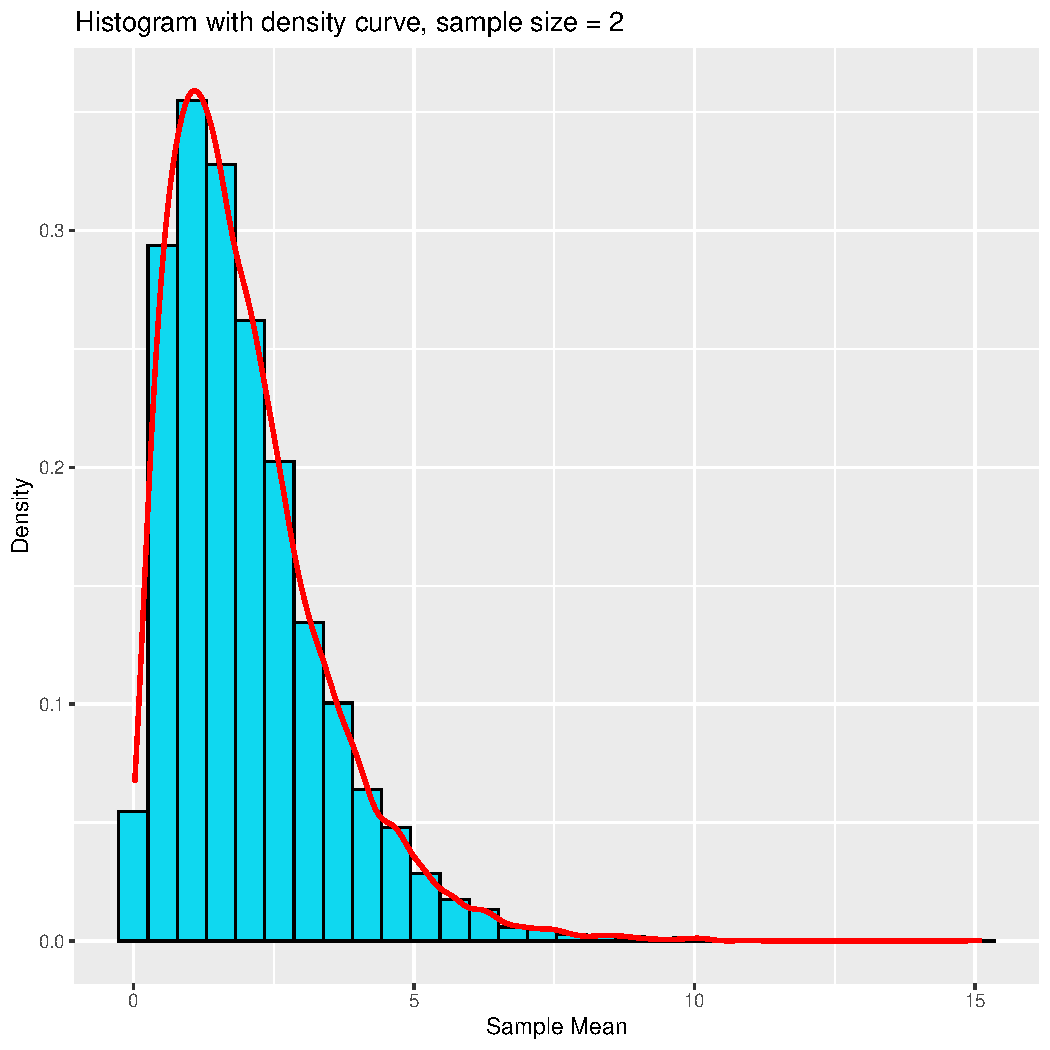
\includegraphics[width=\maxwidth]{figure/unnamed-chunk-7-1} 
\end{knitrout}

\newpage

Next we take $n = 5$.

\begin{knitrout}
\definecolor{shadecolor}{rgb}{0.969, 0.969, 0.969}\color{fgcolor}\begin{kframe}
\begin{alltt}
\hldef{sample_list} \hlkwb{<-} \hlkwd{list}\hldef{(); size} \hlkwb{<-} \hlnum{5}

\hlkwa{for}\hldef{(i} \hlkwa{in} \hlnum{1}\hlopt{:}\hlnum{10000}\hldef{)\{}
  \hldef{sample_list[[i]]} \hlkwb{<-} \hlkwd{rexp}\hldef{(size,} \hlkwc{rate} \hldef{=} \hlnum{1} \hlopt{/} \hldef{theta)}
\hldef{\}}

\hldef{x_bar} \hlkwb{<-} \hlkwd{sapply}\hldef{(sample_list, mean)}
\end{alltt}
\end{kframe}
\end{knitrout}

\begin{knitrout}
\definecolor{shadecolor}{rgb}{0.969, 0.969, 0.969}\color{fgcolor}\begin{kframe}
\begin{alltt}
\hldef{df2} \hlkwb{<-} \hlkwd{data.frame}\hldef{(}\hlkwc{means} \hldef{= x_bar)}

\hldef{df2} \hlopt
  \hlkwd{ggplot}\hldef{(}\hlkwd{aes}\hldef{(}\hlkwc{x} \hldef{= means))} \hlopt{+}
  \hlkwd{geom_histogram}\hldef{(}\hlkwd{aes}\hldef{(}\hlkwc{y} \hldef{= ..density..),} \hlkwc{bins} \hldef{=} \hlnum{30}\hldef{,} \hlkwc{fill} \hldef{=} \hlsng{"#0FD8F0"}\hldef{,} \hlkwc{col} \hldef{=} \hlsng{"black"}\hldef{)} \hlopt{+}
  \hlkwd{geom_density}\hldef{(}\hlkwc{col} \hldef{=} \hlsng{"red"}\hldef{,} \hlkwc{linewidth} \hldef{=} \hlnum{1}\hldef{)} \hlopt{+}
  \hlkwd{labs}\hldef{(}\hlkwc{x} \hldef{=} \hlsng{"Sample Mean"}\hldef{,} \hlkwc{y} \hldef{=} \hlsng{"Density"}\hldef{,}
       \hlkwc{title} \hldef{=} \hlsng{"Histogram with density curve, sample size = 5"}\hldef{)}
\end{alltt}
\end{kframe}
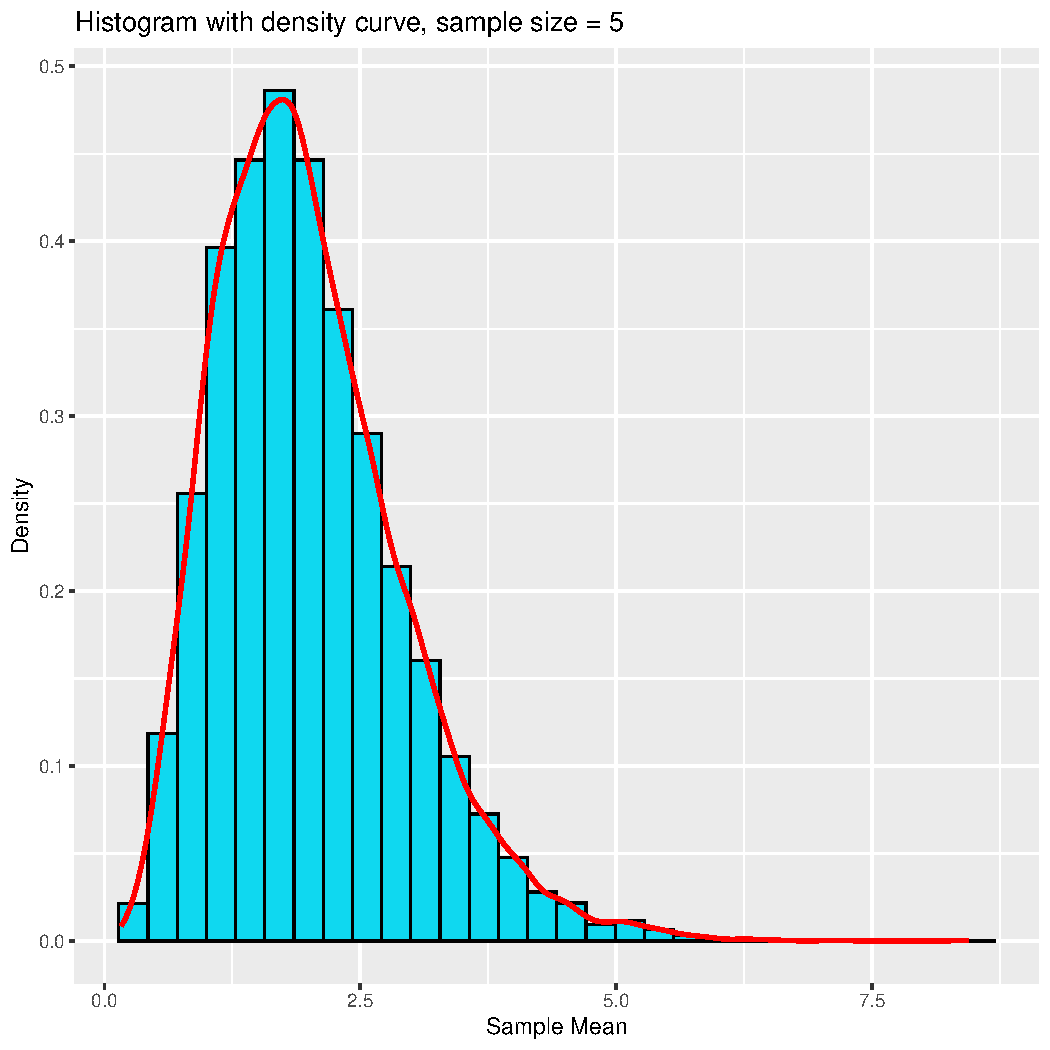
\includegraphics[width=\maxwidth]{figure/unnamed-chunk-9-1} 
\end{knitrout}


\newpage

Next we take $n = 10$.

\begin{knitrout}
\definecolor{shadecolor}{rgb}{0.969, 0.969, 0.969}\color{fgcolor}\begin{kframe}
\begin{alltt}
\hldef{sample_list} \hlkwb{<-} \hlkwd{list}\hldef{(); size} \hlkwb{<-} \hlnum{10}

\hlkwa{for}\hldef{(i} \hlkwa{in} \hlnum{1}\hlopt{:}\hlnum{10000}\hldef{)\{}
  \hldef{sample_list[[i]]} \hlkwb{<-} \hlkwd{rexp}\hldef{(size,} \hlkwc{rate} \hldef{=} \hlnum{1} \hlopt{/} \hldef{theta)}
\hldef{\}}

\hldef{x_bar} \hlkwb{<-} \hlkwd{sapply}\hldef{(sample_list, mean)}
\end{alltt}
\end{kframe}
\end{knitrout}

\begin{knitrout}
\definecolor{shadecolor}{rgb}{0.969, 0.969, 0.969}\color{fgcolor}\begin{kframe}
\begin{alltt}
\hldef{df2} \hlkwb{<-} \hlkwd{data.frame}\hldef{(}\hlkwc{means} \hldef{= x_bar)}

\hldef{df2} \hlopt
  \hlkwd{ggplot}\hldef{(}\hlkwd{aes}\hldef{(}\hlkwc{x} \hldef{= means))} \hlopt{+}
  \hlkwd{geom_histogram}\hldef{(}\hlkwd{aes}\hldef{(}\hlkwc{y} \hldef{= ..density..),} \hlkwc{bins} \hldef{=} \hlnum{30}\hldef{,} \hlkwc{fill} \hldef{=} \hlsng{"#0FD8F0"}\hldef{,} \hlkwc{col} \hldef{=} \hlsng{"black"}\hldef{)} \hlopt{+}
  \hlkwd{geom_density}\hldef{(}\hlkwc{col} \hldef{=} \hlsng{"red"}\hldef{,} \hlkwc{linewidth} \hldef{=} \hlnum{1}\hldef{)} \hlopt{+}
  \hlkwd{labs}\hldef{(}\hlkwc{x} \hldef{=} \hlsng{"Sample Mean"}\hldef{,} \hlkwc{y} \hldef{=} \hlsng{"Density"}\hldef{,}
       \hlkwc{title} \hldef{=} \hlsng{"Histogram with density curve, sample size = 10"}\hldef{)}
\end{alltt}
\end{kframe}
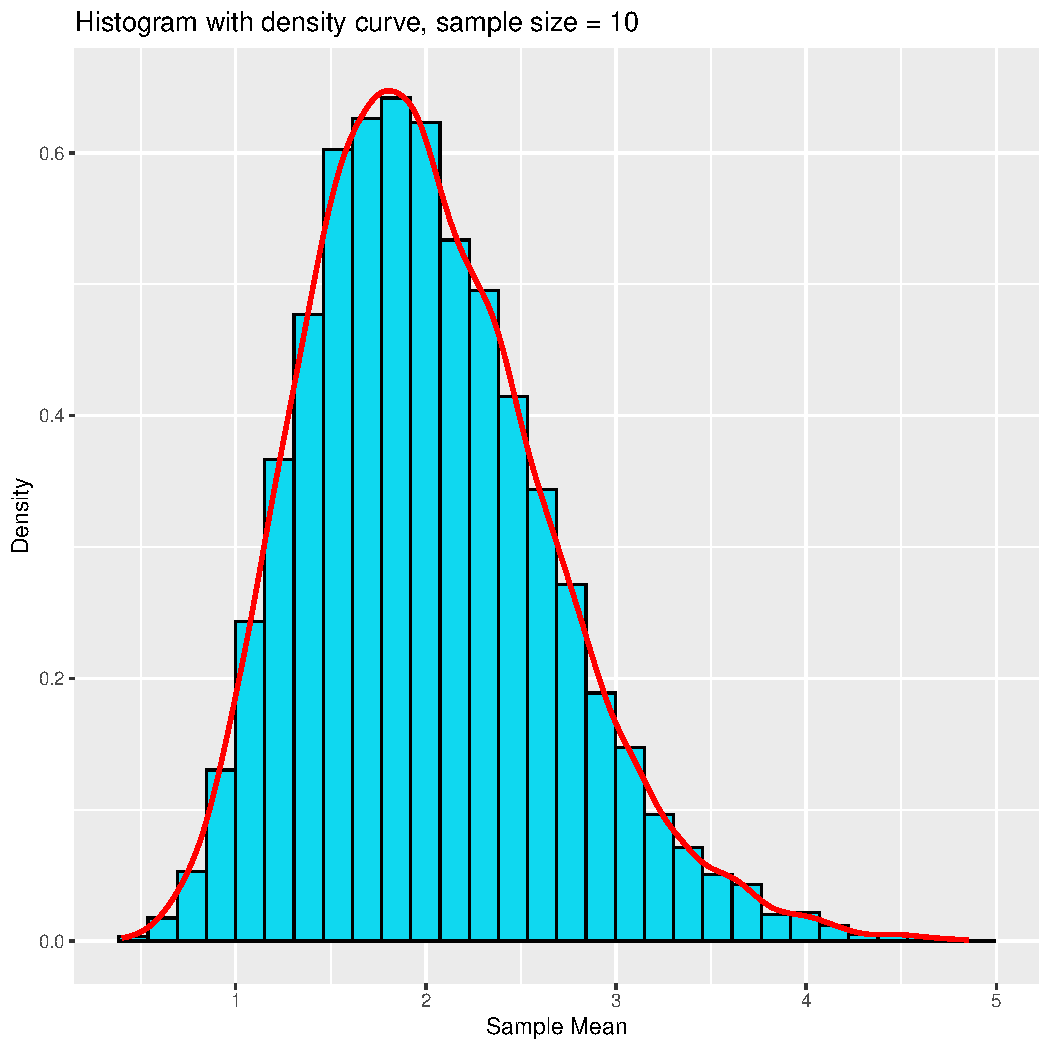
\includegraphics[width=\maxwidth]{figure/unnamed-chunk-11-1} 
\end{knitrout}


\newpage

Finally we take $n = 20$.

\begin{knitrout}
\definecolor{shadecolor}{rgb}{0.969, 0.969, 0.969}\color{fgcolor}\begin{kframe}
\begin{alltt}
\hldef{sample_list} \hlkwb{<-} \hlkwd{list}\hldef{(); size} \hlkwb{<-} \hlnum{20}

\hlkwa{for}\hldef{(i} \hlkwa{in} \hlnum{1}\hlopt{:}\hlnum{10000}\hldef{)\{}
  \hldef{sample_list[[i]]} \hlkwb{<-} \hlkwd{rexp}\hldef{(size,} \hlkwc{rate} \hldef{=} \hlnum{1} \hlopt{/} \hldef{theta)}
\hldef{\}}

\hldef{x_bar} \hlkwb{<-} \hlkwd{sapply}\hldef{(sample_list, mean)}
\end{alltt}
\end{kframe}
\end{knitrout}

\begin{knitrout}
\definecolor{shadecolor}{rgb}{0.969, 0.969, 0.969}\color{fgcolor}\begin{kframe}
\begin{alltt}
\hldef{df2} \hlkwb{<-} \hlkwd{data.frame}\hldef{(}\hlkwc{means} \hldef{= x_bar)}

\hldef{df2} \hlopt
  \hlkwd{ggplot}\hldef{(}\hlkwd{aes}\hldef{(}\hlkwc{x} \hldef{= means))} \hlopt{+}
  \hlkwd{geom_histogram}\hldef{(}\hlkwd{aes}\hldef{(}\hlkwc{y} \hldef{= ..density..),} \hlkwc{bins} \hldef{=} \hlnum{30}\hldef{,} \hlkwc{fill} \hldef{=} \hlsng{"#0FD8F0"}\hldef{,} \hlkwc{col} \hldef{=} \hlsng{"black"}\hldef{)} \hlopt{+}
  \hlkwd{geom_density}\hldef{(}\hlkwc{col} \hldef{=} \hlsng{"red"}\hldef{,} \hlkwc{linewidth} \hldef{=} \hlnum{1}\hldef{)} \hlopt{+}
  \hlkwd{labs}\hldef{(}\hlkwc{x} \hldef{=} \hlsng{"Sample Mean"}\hldef{,} \hlkwc{y} \hldef{=} \hlsng{"Density"}\hldef{,}
       \hlkwc{title} \hldef{=} \hlsng{"Histogram with density curve, sample size = 20"}\hldef{)}
\end{alltt}
\end{kframe}
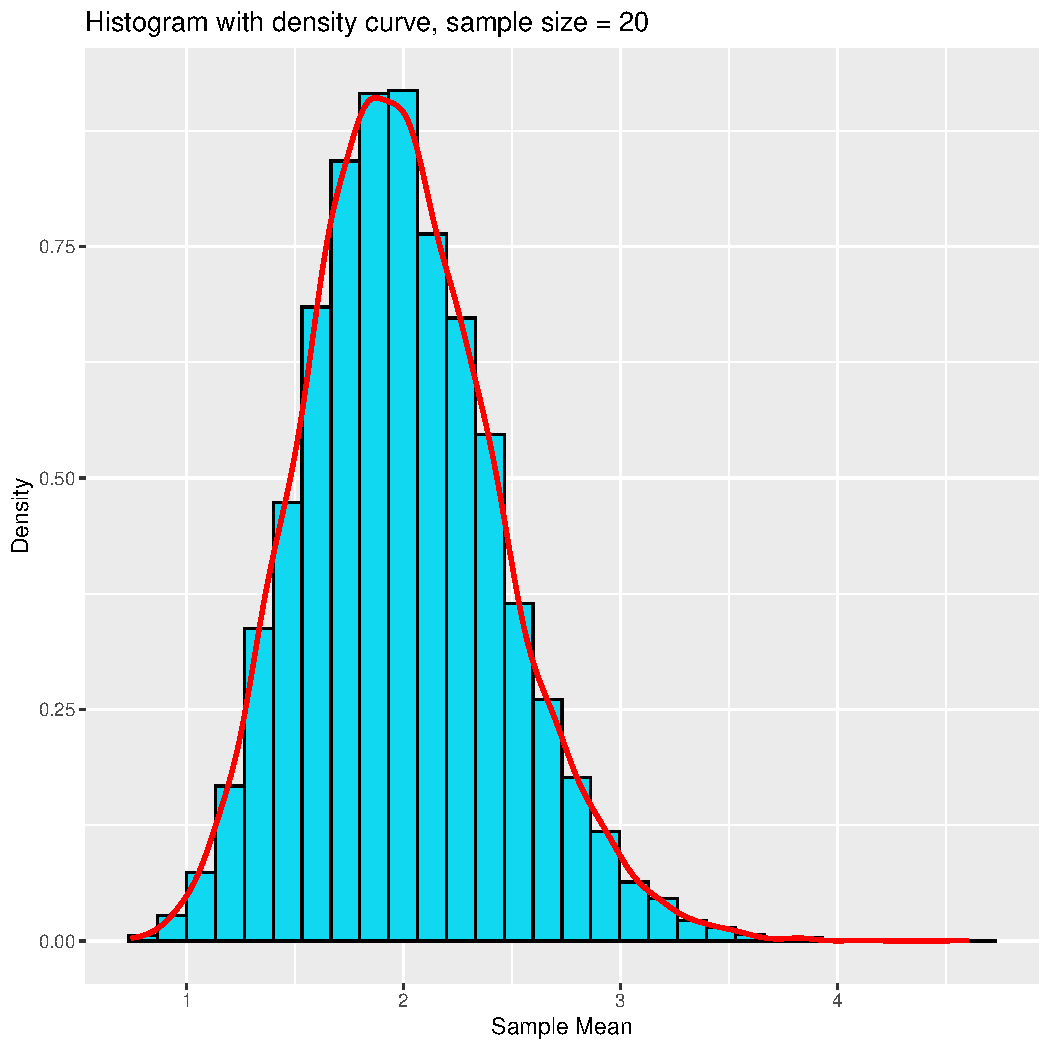
\includegraphics[width=\maxwidth]{figure/unnamed-chunk-13-1} 
\end{knitrout}

\smallpencil {\setlength{\spaceskip}{1em plus 0.5em minus 0.5em} \fontsize{17}{20}\myfont The density curve has pretty much resemblance with that of a normal density curve, thus implying convergence in distribution of the sample mean. \par}

{\setlength{\spaceskip}{1em plus 0.5em minus 0.5em} \fontsize{17}{20}\myfont Hence it is established that the sample mean is a CAN estimator for $\theta$. \par}

\vspace{1cm}

\leftpointright \hspace{0.5cm} Now we have to obtain a CAN estimator for $\psi{(\theta)} = e^{-t/ \theta}$. $\psi{(\theta)}$ is differentiable function of $\theta$, $\dfrac{d\psi}{d\theta}$ is non-vanishing and continuous. We already have $\bar{X}$ is a CAN estimator for $\theta$. Thus by invariance property of a CAN estimator, $\psi{(\bar{X})}$ is a CAN estimator of $\psi{(\theta)}$ and 
$$\psi{(\bar{X})} \sim AN \left(\psi{(\theta)}, \dfrac{\theta^2}{n} \left( \dfrac{d\psi}{d\theta} \right)^2 \right).$$

So asymptotic variance of $\psi{(\bar{X})}$ is $\dfrac{t^2}{n \theta^2} e^{-2t / \theta}.$ \\

Here we take $t = 1$ and $\theta = 2$. \\

So $\psi{(\theta)} = 0.6065307$.

\begin{knitrout}
\definecolor{shadecolor}{rgb}{0.969, 0.969, 0.969}\color{fgcolor}\begin{kframe}
\begin{alltt}
\hldef{estimate} \hlkwb{<-} \hlkwa{function}\hldef{(}\hlkwc{n}\hldef{)} \hlkwd{return}\hldef{(}\hlkwd{exp}\hldef{(}\hlopt{-}\hlnum{1}\hlopt{/}\hlkwd{mean}\hldef{(}\hlkwd{rexp}\hldef{(n,} \hlkwc{rate} \hldef{=} \hlnum{1}\hlopt{/}\hlnum{2}\hldef{))))}

\hldef{asv} \hlkwb{<-} \hlkwa{function}\hldef{(}\hlkwc{n}\hldef{)} \hlkwd{return}\hldef{(}\hlkwd{exp}\hldef{(}\hlopt{-}\hlnum{1}\hldef{)} \hlopt{/} \hldef{(n} \hlopt{*} \hlnum{4}\hldef{))}
\end{alltt}
\end{kframe}
\end{knitrout}

\begin{knitrout}
\definecolor{shadecolor}{rgb}{0.969, 0.969, 0.969}\color{fgcolor}\begin{kframe}
\begin{alltt}
\hldef{df3} \hlkwb{<-} \hlkwd{data.frame}\hldef{(}\hlkwc{sample_size} \hldef{=} \hlkwd{seq}\hldef{(}\hlnum{5}\hldef{,} \hlnum{50}\hldef{,} \hlnum{5}\hldef{),}
                  \hlkwc{estimated_psi_theta} \hldef{=} \hlkwd{sapply}\hldef{(}\hlkwd{seq}\hldef{(}\hlnum{5}\hldef{,} \hlnum{50}\hldef{,} \hlnum{5}\hldef{),} \hlkwc{FUN} \hldef{= estimate),}
                  \hlkwc{variance} \hldef{=} \hlkwd{asv}\hldef{(}\hlkwd{seq}\hldef{(}\hlnum{5}\hldef{,} \hlnum{50}\hldef{,} \hlnum{5}\hldef{)))}
\hldef{df3}
\end{alltt}
\begin{verbatim}
##    sample_size estimated_psi_theta    variance
## 1            5           0.3734812 0.018393972
## 2           10           0.5506846 0.009196986
## 3           15           0.5726035 0.006131324
## 4           20           0.6453451 0.004598493
## 5           25           0.6252023 0.003678794
## 6           30           0.6857392 0.003065662
## 7           35           0.4983047 0.002627710
## 8           40           0.5112385 0.002299247
## 9           45           0.5741369 0.002043775
## 10          50           0.5627382 0.001839397
\end{verbatim}
\end{kframe}
\end{knitrout}

\smallpencil {\setlength{\spaceskip}{1em plus 0.5em minus 0.5em} \fontsize{17}{20}\myfont Thus we get estimates of the parametric function for different sample sizes. The variance of the estimate decreases as sample size increases. \par}


\end{document}
